\page{
  疲れましたか。
}{
  ええ、
  ちょっとだけ。
}

\page{休憩のつもりで散歩をしましょう}
{夕方の散策ですね}

\page{
  前回、私が最後になんと言ったか、
覚えてますか。}
{
  ええ、
任意のユニタリー変換を施すことができると言いました}

\page{
  次は、ユニタリー変換ですか。
  $$\ket{i} \mapsto \ket{i-1} + \ket{i+1}$$
}
{
  聞きたいことが2つほどあるのですが。
}

\page{
  もちろん!
  時間はまだまだありますよ。
}
{
  まず、見た目が行列になっていないのですが
}

\page{
  ささいな問題です!
  実際、次のようにして、簡単に行列にできます。
  $i$ 番目だけが $1$ で他が $0$ な列ベクトル:
  $$( 0 ... 0, 1, 0 ... 0 )^\top$$
  これが $\ket{i}$ の正体です。
  $$U \ket{i} = \ket{i-1} + \ket{i+1}$$
  となればよいのですが、
  左辺は $U$ の第 $i$ 列目であることがわかります。
}{
  ふたつ目の質問ですが、
  では、$i$ の範囲を教えてください。
}

\page{
  自然数全体 $\mathbb{Z}$ としましょう。
}{
  ええ、それは無限にありますよ。
  無限の qビットが必要になってしまいます!
}

\page{
大丈夫、有限しか使いません。}
{先ほどの変換の行列バージョンをくれますか。}

\page{
  $$
  U =
  \left( \begin{array}{ccccc}
      \ddots \\
             & 1 \\
             & 0 & 1 \\
             & 1 & 0 & 1 \\
             &   & 1 & 0 \\
             &   &   & 1 \\
             &   &   &  & \ddots
  \end{array} \right)
  $$
}{
  $$U_{ij} = \begin{cases}
    1 & i-j = \pm 1 \text{ のとき}\\
    0
  \end{cases}$$
}

\page{
  これはユニタリー行列ですか。
}{
  $u_i^* u_i = 1^2 + 1^2$
  なので違います。
}

\page{
  では
  $\frac{1}{\sqrt{2}}U$
  はユニタリー行列ですか。
}{
  $u_i^* u_{i+2} = 1$
  なので違います。
}

\page{
  $$\ket{i} \mapsto \frac{1}{\sqrt{2}}\ket{i-1} + \frac{1}{\sqrt{2}}\ket{i+1}$$
  の意味はわかりますか。
}{
  50\%の確率で $\ket{i}$ が $\ket{i-1}$ になります。
  50\%の確率で $\ket{i}$ が $\ket{i+1}$ になります。
  でもユニタリー変換ではないので、不当な操作です。
}

\page{
  どうしたらよいでしょうか。
}{
  もっと行列をスパースにすればよいと思います。
}

\page{
  アイデアを借りてもよろしいですか。
}{
  縦にスパースにします。
  先ほどの行列 $U$ で $1$ があった行のすぐ下に
  全て $0$ で満たされた行を挿入します。
  $$
  \left( \begin{array}{ccccc}
      \ddots \\
             & 1 \\
             & \bf{0} \\
             & 0 & 1 \\
             &   & \bf{0} \\
             & 1 & 0 & 1 \\
             & \bf{0} &   & \bf{0} \\
             &   & 1 & 0 \\
             &   & \bf{0} &   \\
             &   &   & 1 \\
             &   &   & \bf{0} \\
             &   &   &  & \ddots
  \end{array} \right)
  $$
}

\page{
  なるほど、
  $1$ がずれたので
  別な列を掛けると$0$になりますね。\\
  でも行列は$n \times n$ の正方行列でないといけませんよ。
}{
  列は次のように挿入します。
  $$
  \left( \begin{array}{ccccccccc}
      \ddots \\
         & 1 & \bf{1} \\
         & 0 & \bf{0} \\
         & 0 & \bf{0} & 1 & \bf{1} \\
         &   & \bf{ } & 0 & \bf{0} \\
         & 1 & \bf{-1} & 0 & \bf{0} & 1 & \bf{1} \\
         & 0 & \bf{0} &   & \bf{ } & 0 & \bf{0} \\
         &   &   & 1 & \bf{-1} & 0 & \bf{0} \\
         &   &   & 0 & \bf{0} &   & \bf{ } \\
         &   &   &   &   & 1 & \bf{-1} \\
         &   &   &   &   & 0 & \bf{0} \\
         &   &   &   &   &   &   & \ddots
  \end{array} \right)
  $$
  これを $\frac{1}{\sqrt{2}}$ 倍した変換を考えます。
}

\page{
  確かにユニタリーですね。
  でも、どう読み取れば?
}{
  $\ket{i}$ に2種類の ``タグ'' を付け加えます。
  $\ket{i, 0}$ と $\ket{i, 1}$ です。
  $$\ket{i, 0} \mapsto \frac{1}{\sqrt{2}}\ket{i-1, 0} + \frac{1}{\sqrt{2}}\ket{i+1, 1}$$
  $$\ket{i, 1} \mapsto \frac{1}{\sqrt{2}}\ket{i-1, 0} - \frac{1}{\sqrt{2}}\ket{i+1, 1}$$
}

\page{
  $\ket{i, 0} \mapsto \ket{i}$、 $\ket{i, 1} \mapsto \ket{i}$
  と読み替えれば、確かに
  先ほどの変換と一致します!
}{
  定義してみます。
  この変換はなんという名前にしますか。
}

\page{
  \v{random-walk}
  と名づけましょう
}{
  そういえば先程は、取りうる状態 $\ket{i} (i = 0,1,\ldots,n-1)$ の
  種類の数を長さにしたリストにしましたが、
  今回は無限あります。
}



\hline
\begin{minipage}{.01\hsize}
  ~
\end{minipage}
\begin{minipage}{.39\hsize}
  有限しか使いません。
  十分大きくとればよいでしょう。
  また、
  $$\ket{i, 0} \equiv \ket{2i}, \ket{i,1} \equiv \ket{2i+1}$$
  と便宜的にしておくと扱いやすそうです。
\end{minipage}
\begin{minipage}{.10\hsize}
  ~
\end{minipage}
\begin{minipage}{.39\hsize}
  \begin{verbatim}
(define (nth ls n)
  (if (or (< n 0)
           (>= n (length ls)))
    0
    (ref ls n)))

(define (random-walk p)
  (map (lambda (i)
    (if (even? i)
      (+ (nth p (+ i 2))
         (nth p (+ i 3)))
      (- (nth p (- i 3))
         (nth p (- i 2)))))
    (iota (length p))))
  \end{verbatim}
\end{minipage}

\page{
  \v{nth} はなんですか
}{
  範囲外アクセスしようとすると $0$を返すようなアクセサです
}

\page{
本当は最後に \v{/sqrt2} 倍しないといけませんけどね}
{心の目}



\hline
\begin{minipage}{.01\hsize}
  ~
\end{minipage}
\begin{minipage}{.39\hsize}
  \begin{verbatim}
(define (times n f x)
  (if (positive? n)
    (begin
      (print x)
      (times (- n 1) f (f x)))))
  \end{verbatim}
\end{minipage}
\begin{minipage}{.10\hsize}
  ~
\end{minipage}
\begin{minipage}{.39\hsize}
  最初の多qビットの発生源も必要です!
\end{minipage}



\hline
\begin{minipage}{.01\hsize}
  ~
\end{minipage}
\begin{minipage}{.39\hsize}
  \begin{verbatim}
(define (random-qs n)
  (let* ((qs
          (map (^_ (- (random-real)
                      0.5))
               (iota n)))
         (Z
          (sqrt (apply +
                  (map (^x (* x x))
                       qs)))))
      (map (cut / <> Z) qs)))
  \end{verbatim}
\end{minipage}
\begin{minipage}{.10\hsize}
  ~
\end{minipage}
\begin{minipage}{.39\hsize}
  \begin{verbatim}
gosh> (random-qs 10)
(0.21311994855400265 0.4540140911161344
-0.36816606569943633 0.2813168420814456
-0.19153946328486496 -0.4673264315974541
-0.3657098841566678 0.13189203266396135
0.35711782508621465 0.0034564021126312796)
gosh> (observe (random-qs 10))
(0 1 0 0 0 0 0 0 0 0)
  \end{verbatim}
\end{minipage}



\hline
\begin{minipage}{.01\hsize}
  ~
\end{minipage}
\begin{minipage}{.39\hsize}
  良さそうですね。続けてください。
\end{minipage}
\begin{minipage}{.10\hsize}
  ~
\end{minipage}
\begin{minipage}{.39\hsize}
\end{minipage}

\begin{verbatim}
gosh> (times 10 random-walk (observe (random-qs 30)))
(0 0 0 0 0 0 0 0 0 0 0 0 0 0 0 0 0 0 0 0 0 0 0 0 0 0 0 1 0 0)
(0 0 0 0 0 0 0 0 0 0 0 0 0 0 0 0 0 0 0 0 0 0 0 0 1 0 0 0 0 -1)
(0 0 0 0 0 0 0 0 0 0 0 0 0 0 0 0 0 0 0 0 0 0 1 0 0 0 -1 1 0 0)
(0 0 0 0 0 0 0 0 0 0 0 0 0 0 0 0 0 0 0 0 1 0 0 0 0 1 0 0 0 -2)
(0 0 0 0 0 0 0 0 0 0 0 0 0 0 0 0 0 0 1 0 0 0 1 1 0 0 -2 -1 0 0)
(0 0 0 0 0 0 0 0 0 0 0 0 0 0 0 0 1 0 0 0 2 1 0 0 -3 0 0 0 0 -1)
(0 0 0 0 0 0 0 0 0 0 0 0 0 0 1 0 0 0 3 1 0 0 -3 1 0 0 -1 -3 0 0)
(0 0 0 0 0 0 0 0 0 0 0 0 1 0 0 0 4 1 0 0 -2 2 0 0 -4 -4 0 0 0 2)
(0 0 0 0 0 0 0 0 0 0 1 0 0 0 5 1 0 0 0 3 0 0 -8 -4 0 0 2 0 0 0)
(0 0 0 0 0 0 0 0 1 0 0 0 6 1 0 0 3 4 0 0 -12 -3 0 0 2 -4 0 0 0 2)
#<undef>
gosh> (times 10 random-walk (observe (random-qs 30)))
(0 0 0 0 0 0 0 0 0 0 0 0 0 0 0 1 0 0 0 0 0 0 0 0 0 0 0 0 0 0)
(0 0 0 0 0 0 0 0 0 0 0 0 1 0 0 0 0 -1 0 0 0 0 0 0 0 0 0 0 0 0)
(0 0 0 0 0 0 0 0 0 0 1 0 0 0 -1 1 0 0 0 1 0 0 0 0 0 0 0 0 0 0)
(0 0 0 0 0 0 0 0 1 0 0 0 0 1 0 0 1 -2 0 0 0 -1 0 0 0 0 0 0 0 0)
(0 0 0 0 0 0 1 0 0 0 1 1 0 0 -1 -1 0 0 -1 3 0 0 0 1 0 0 0 0 0 0)
(0 0 0 0 1 0 0 0 2 1 0 0 -2 0 0 0 2 0 0 0 1 -4 0 0 0 -1 0 0 0 0)
(0 0 1 0 0 0 3 1 0 0 -2 1 0 0 2 -2 0 0 -3 2 0 0 -1 5 0 0 0 1 0 0)
(1 0 0 0 4 1 0 0 -1 2 0 0 0 -3 0 0 -1 4 0 0 4 -5 0 0 1 -6 0 0 0 -1)
(0 0 5 1 0 0 1 3 0 0 -3 -3 0 0 3 3 0 0 -1 -5 0 0 -5 9 0 0 -1 7 0 0)
(6 0 0 0 4 4 0 0 -6 -2 0 0 6 0 0 0 -6 0 0 0 4 4 0 0 6 -14 0 0 0 -8)
#<undef>
gosh> (times 10 random-walk (observe (random-qs 30)))
(0 0 0 0 0 0 0 0 0 0 0 0 0 0 0 0 0 0 0 0 0 0 0 0 1 0 0 0 0 0)
(0 0 0 0 0 0 0 0 0 0 0 0 0 0 0 0 0 0 0 0 0 0 1 0 0 0 0 1 0 0)
(0 0 0 0 0 0 0 0 0 0 0 0 0 0 0 0 0 0 0 0 1 0 0 0 1 1 0 0 0 -1)
(0 0 0 0 0 0 0 0 0 0 0 0 0 0 0 0 0 0 1 0 0 0 2 1 0 0 -1 0 0 0)
(0 0 0 0 0 0 0 0 0 0 0 0 0 0 0 0 1 0 0 0 3 1 0 0 -1 1 0 0 0 -1)
(0 0 0 0 0 0 0 0 0 0 0 0 0 0 1 0 0 0 4 1 0 0 0 2 0 0 -1 -2 0 0)
(0 0 0 0 0 0 0 0 0 0 0 0 1 0 0 0 5 1 0 0 2 3 0 0 -3 -2 0 0 0 1)
(0 0 0 0 0 0 0 0 0 0 1 0 0 0 6 1 0 0 5 4 0 0 -5 -1 0 0 1 -1 0 0)
(0 0 0 0 0 0 0 0 1 0 0 0 7 1 0 0 9 5 0 0 -6 1 0 0 0 -4 0 0 0 2)
(0 0 0 0 0 0 1 0 0 0 8 1 0 0 14 6 0 0 -5 4 0 0 -4 -7 0 0 2 4 0 0)
#<undef>
\end{verbatim}

\page{
}{
  左に ``寄って'' いるように見えるのですが。
}
\page{
  気のせいではありませんか。
}{
  気のせいではなさそうです!
}
\begin{verbatim}
gosh> (times 10 random-walk '(0 0 0 0 0 0 0 0 0 0 1 0 0 0 0 0 0 0 0 0 0))
(0 0 0 0 0 0 0 0 0 0 1 0 0 0 0 0 0 0 0 0 0)
(0 0 0 0 0 0 0 0 1 0 0 0 0 1 0 0 0 0 0 0 0)
(0 0 0 0 0 0 1 0 0 0 1 1 0 0 0 -1 0 0 0 0 0)
(0 0 0 0 1 0 0 0 2 1 0 0 -1 0 0 0 0 1 0 0 0)
(0 0 1 0 0 0 3 1 0 0 -1 1 0 0 1 -1 0 0 0 -1 0)
(1 0 0 0 4 1 0 0 0 2 0 0 0 -2 0 0 -1 2 0 0 0)
(0 0 5 1 0 0 2 3 0 0 -2 -2 0 0 1 2 0 0 0 -3 0)
(6 0 0 0 5 4 0 0 -4 -1 0 0 3 0 0 0 -3 -1 0 0 0)
(0 0 9 6 0 0 -5 1 0 0 3 -3 0 0 -4 3 0 0 0 -2 0)
(15 0 0 0 -4 3 0 0 0 -6 0 0 -1 6 0 0 -2 -7 0 0 0)
#<undef>
\end{verbatim}


\hline
\begin{minipage}{.01\hsize}
  ~
\end{minipage}
\begin{minipage}{.39\hsize}
  実験してみましょう。
  $\ket{i}$ を観測する確率は、今は、
  $\ket{i,0}$ を観測する確率と
  $\ket{i,1}$ を観測する確率との和なので、
  状態から確率それぞれを観測できる確率のリストへ次を使って変換できます。
  \v{compress}
\begin{verbatim}
(define (compress x)
  (if (< (length x) 2)
    '()
    (cons (+ (expt (car x) 2)
             (expt (cadr x) 2))
          (compress (cddr x)))))
\end{verbatim}
\end{minipage}
\begin{minipage}{.10\hsize}
  ~
\end{minipage}
\begin{minipage}{.39\hsize}
\begin{verbatim}
gosh> (plot-times 10 random-walk
'(0 0 0 0 0 0 0 0 0 0
  1 0
  0 0 0 0 0 0 0 0 0 0))
\end{verbatim}
\end{minipage}

\hline

  \begin{verbatim}
(use gauche.process)
(define (show xs out) ; 折れ線グラフの描画
  (call-with-output-process "/usr/bin/gnuplot" (lambda (port)
    (display #`"set terminal png; set output \",out\";" port)
    (display "plot \"-\" w lp\n" port)
    (for-each (cut format port "~a\n" <>) xs))))


(define (plot-times n f x)
  (let loop ((i 0) (x x))
    (when (< i n)
      (show (compress x) #`",|i|.png")
      (loop (+ i 1) (f x)))))
\end{verbatim}

\begin{center}
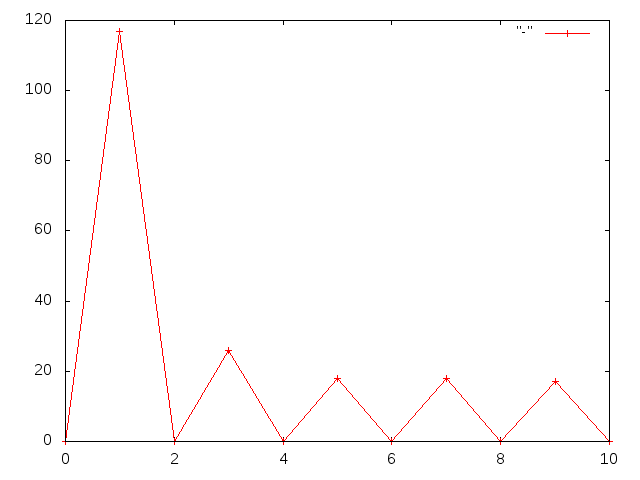
\includegraphics[width=1.0\textwidth,bb=0 0 640 480]{img/8.png}
\text{8.png}
\end{center}

\page{
  ところで知らない道に出てしまいました。
  帰り道を覚えていますか。
}{
  …。
}

